%@+leo-ver=4-thin
%@+node:rodrigob.20040908003956.1:@thin doc/design_proposal.tex
%@@color
%@@language latex

%\documentclass{report}
\documentclass{article}
%\documentclass[A4paper, notitlepage]{article}
                                              
\usepackage[utf8]{inputenc}
\usepackage[english]{babel}
\usepackage{graphicx}
\usepackage{verbatim}

\frenchspacing
\linespread{1} %espacio entre líneas
%\setlength{\parindent}{25pt} %profundidad de la sangría
\setlength{\parskip}{0.7ex plus 0.2ex minus 0.2ex} %espacio entre párrafos

\usepackage{fancyhdr}
\usepackage[sectionbib]{chapterbib}
\usepackage{amsmath}

\usepackage[pdftex]{hyperref}


\lhead{Chalks}
\rhead{\emph{Design proposal}}
\lfoot{}
\cfoot{\thepage}
\rfoot{}

%\usepackage[top=2cm,bottom=2cm,left=2.5cm,right=2.5cm,footskip=1cm,headheight=.5cm,headsep=2cm,textheight=3cm]{geometry}
\usepackage[top=2cm,bottom=2cm,left=2.5cm,right=2.5cm]{geometry}
                                              
\pagestyle{fancy}

\title{\large Chalks \\ \huge Design proposal}
\author{Rodrigo Benenson, Ricardo Niederberger}
\date{Technical draft as of\\ \today}

                                           
\begin{document}


\begin{figure}[!t]
 \begin{center}
    
\includegraphics[angle=0,width=5cm]{schemas/logo.jpg}
 \end{center}
\end{figure}


\maketitle
\thispagestyle{empty}

\newpage
\setcounter{page}{1}


\tableofcontents
\newpage
%@+at
% \listoffigures
% %\newpage
% 
% \listoftables
% \newpage
%@-at
%@@c

%@+others
%@+node:rodrigob.20040908004801:Introduction
\section{Introduction}

This text covers every defined \href{http://ryalias.freezope.org/Chalks/Aspects}{aspect} and propose a technical solution to implement the \href{http://ryalias.freezope.org/Chalks/ChalksRequirements}{requirements}.
This is mostly a documentation of the inicial Chalks design.


Root concept: \emph{Keep It Simple}, minimal complexity to acomplish the strictly necessary requirements.


%@-node:rodrigob.20040908004801:Introduction
%@+node:rodrigob.20040908010357:Concurrent Editing
\section{Concurrent Editing}

Direct implementation of the linear undo/redo algorithm described in Chengzheng Sun's works. This algorithm is the simpler aviable. It has a good compromise in the memory/cpu usage, with a some charge on the memory. Anyway as the objects managed are strings, the memory rarely grows more than a few tens of megabytes.

Chengzheng Sun's algorithm define three objects: the operations, the history buffer (HB), and the resulting text.

The operations are specific transformation over the text (insertion, deletion) originated from a specific version of the text. The history buffer is a buffer of all the operations applied over the text. And the resulting text is the consecuence of applying all the HB operations over the original text.

The concurrent editable algorithm define what to do with an new operations. The processing of the received operations will have effect over the HB and over the original resulting text.


\begin{figure}[htbp]
 \begin{center}
    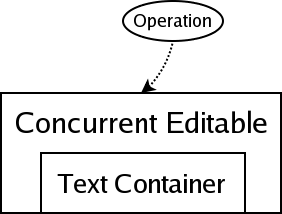
\includegraphics[angle=0,width=0.5\linewidth]{schemas/concurrent_editable.png}
 \end{center}
 \label{fig:concurrenteditable}
 \caption{ConcurrentEditable, TextContainer and the Operations}
\end{figure}

\fbox{\begin{minipage}[c]{\linewidth}
\emph{Note}: the actual WIP version does not separate in a clear enough way the TextContainer from the ConcurrentEditable object. I think this separation should be enforced to ease later integration with GUI
\end{minipage}}

Using Python power the operations can be easilly represented as objects, following an easy api similar to Chengzheng Sun's notation.

In a similar way the Concurrent Editable algorithm can be implemented as an almost direct translation from the Chengzheng Sun papers to python code.

The {\texttt TextContainer } class is a simple one that contain an unicode string, and have methods for insertion, deletion of chars and the retrieval of the actual content.
%@-node:rodrigob.20040908010357:Concurrent Editing
%@+node:rodrigob.20040908010357.1:Network
\section{Network}

The definition and implementation of the networking system is the most difficult aspect of the software. Distributed bugs arises and issues not covered in the papers have to be afronted.

Essentially the network has to take care of three things:
\begin{itemize}
\item Sent operations have to arrive to every connected user
\item If a new user logs in, everyone has to know about it
\item If a user logs out, everyone has to know about it
\end{itemize}

Every operation has a specific identifier. This identifier is the number of operations that the emitter site has received from other sites (including himself). This identifier defines without ambiguity the *version* of the document over which the operation was generated.

To simplify the implementation instead of enumerating the sites (as in the paper) the sites are individualized by an unique id (ip+port). Then the operations are tagged with a dictionary of the kind {\texttt {id1: ops\_from\_id1, id2: ops\_from\_id2, ...}} (including site own id).

This approach becames less efficient if many sites just connect once, send an operation and then disconnect, but this is a rare case. This approach is less efficient than using an ordered list, but it is simpler and functional. It is simpler because we do not care about the order of arrival, the disconnections and reconnections, and when new users are added to the session the management becomes trivial.

%@+others
%@+node:rodrigob.20040908012337:Topology
\subsection{Network topology}

Following the KIS principle which is the simplest network architectures that does the job fine ?

The proposal is to use a ``Connect to One, Accept N'' topology, also known as a ``simple tree''. See the image \ref{fig:connectooneacceptN} to get an idea.    

\begin{figure}[htbp]
 \begin{center}
    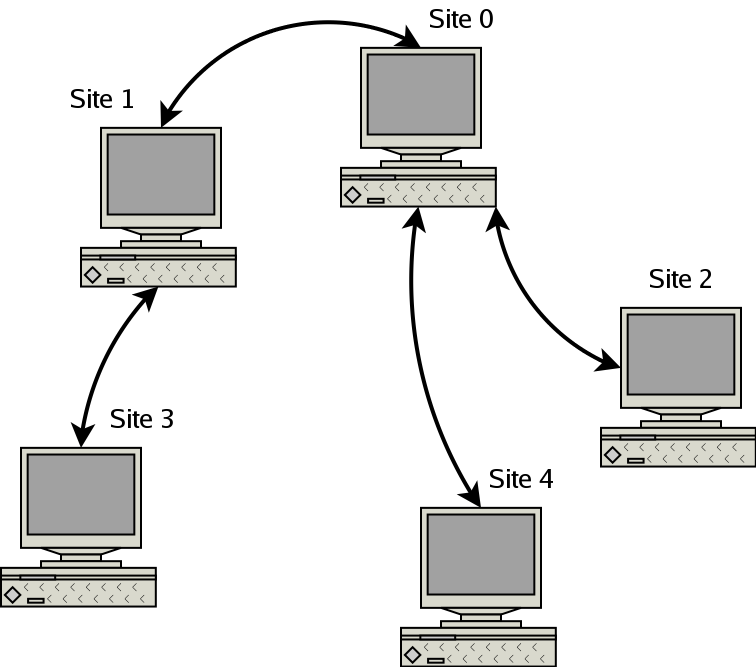
\includegraphics[angle=0,width=0.5\linewidth]{schemas/connect_to_one_accept_N.png}
 \end{center}
 \label{fig:connectooneacceptN}
 \caption{Connect to One, Accept N ilustrative topology}
\end{figure}

The concept of this topology is, very simple. One user only want to connect himself to one computer, so let's do that. If more than one user want to connect to the same computer let's do that. After the first connection no more connections are made.

This is topology is inefficient. In the figure, when site 4 edit the text, the operation will be relayed by site 0 and site 1, adding inecessary delays. This is true, but this topology is very simple implement. It has also an interesant advantage, it gives to the users the control of the network. In the figure, if sites [0,2,4] are in the same LAN, and sites [1,3], in another one, then the topology is not so bad. Also if an user is working in a slow connection (example, low SNR wireless conneciton), it would prefer to have only one connection to the nearest (in ping measure) machine. Having more than one connection add transfers costs to keep the TCP/IP links alive. If the users control the conection they can choose the computer with overload. A tipical user case will be simply N-to-One (central server receiving all the conections).
 
The tree topology is not only simple to implement but also simple to analyse.
    
When a site receives an operation it applies it locally and spread it to all the other known sites, excluding the node that sent the operation. As the topology is an acyclic graph, no special precautions has to be taken (to avoid repeated reception).

Let's see what should happen when a user connects himself to a session.
\begin{itemize}
\item New user enters the network

A user has choosen a machine to connect to. This machine receives a new connection and has to send back, the current text and the HB. We have to take care of new operations that could be generated during the connection process.

Chengzheng Sun's algorithm includes a purge procedure to avoid the HB getting unncessarily big.

This HB purge could be implemented as a method which calls itself repeatedly, using a call like "reactor.callLater(self.HBPurge(), purgeDelay)". This "service method" pattern could repeat a lot on such networked application, especially when using a networking framework like Twisted, with deferred execution.

Upon the first text editing, the new user will generate an operation with a new entry in the tag. When a site receives it for the first time it will include it in the list of know sites. If a received operation does not include (not a key in it's id->version map) a known site id, obviously this node has received zero operations from that site.


\item A user quits the network

No special precaution has to be taken when a user quits. We have to simply disconnect from the parent node, and kill all children nodes. This will create a cascade that will close the branch adequately.


\fbox{\begin{minipage}[c]{\linewidth}
\emph{Note}: this could be an inconvenience, depending of the usage scheme. Maybe we could create a transaction system to invite all children nodes to connect themself to the parent node. But synchronisation issues may arise (``what if a packet arives to the parent while children-childrens are connecting to them ?''). This is a non trivial topic that we should check. For an initial implementation branch die seems fine to me, but is it the desired behaviour ? (let's check the requiriment)
\end{minipage}}

      
HB purge should also purge sites info. If a site id does not appear more in the HB, then it should be deleted from the known sites list, thus shrinking back the packet sizes since no memory traces are keep in any connected site.
\end{itemize}
%@nonl
%@-node:rodrigob.20040908012337:Topology
%@-others

\subsection{Protocol}

{\texttt Operation} objects serialized and transfered via Twisted Spread.

\begin{itemize}
\item Well documented API
\item Simple and eficient binary serialization (low bandwith usage)
\item Well documented Serialization protocol (Banana)
\item Fast serialization (C modules)
\item Pythonic
\end{itemize}

\subsection{API}
  
\href{http://www.twistedmatrix.com}{Twisted}

\begin{itemize}
\item Well documented API
\item Full featured, spread, authentication, web services, diverse protocols, etc.
\item Pythonic
\item Easy to embed in the software distribution
\end{itemize}
%@nonl
%@-node:rodrigob.20040908010357.1:Network
%@+node:rodrigob.20040908010357.2:Gui
\section{Gui}

Show the text container, generate new operations over the text, allow sending chat messages to the other users.

The idea is to provide to the user all what it need to see in only one window, splitted in two areas: the text area and the chat area.

\begin{figure}[htbp]
 \begin{center}
    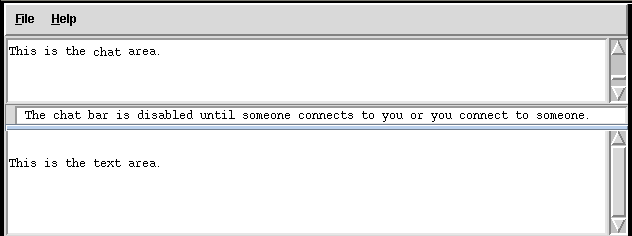
\includegraphics[angle=0,width=0.5\linewidth]{schemas/text_and_chat_area.png}
 \end{center}
 \label{fig:textandchatarea}
 \caption{Text and chat areas in the same window}
\end{figure}

  
The chat area is used as a log window, to receive message, and have an input section to send messages. This input section can also be used to enter advanced commands (to enable/disable debug logs, to select special options, etc...). Different colors in the chat bar are used to differenciate diferent kind of messages.

The chat area is resizable (click and drag). If  it is totally colapsed it transform itself into a status bar, that show the last line in the chat area.

\begin{figure}[htbp]
 \begin{center}
    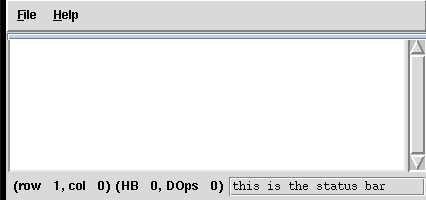
\includegraphics[angle=0,width=0.5\linewidth]{schemas/colapsable_chat_area.png}
 \end{center}
 \label{fig:colapsablechatarea}
 \caption{The chat area is colapsable, transforming itself in a normal status bar}
\end{figure}


In the text area color codes are used to differenciate the users entries. Also the local entry are marked in such a way that the local user know when a group of chars have been sent or not.


\begin{figure}[htbp]
 \begin{center}
    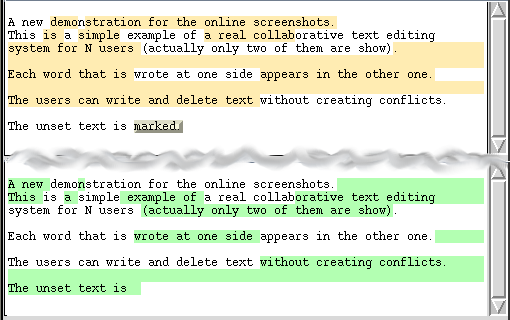
\includegraphics[angle=0,width=0.5\linewidth]{schemas/collaborating_small_shot.png}
 \end{center}
 \label{fig:collaboratingsmallshot}
 \caption{Text from other users are colored. Text not yet processed is raised}
\end{figure}



The color of the users is randomly choosen at the local site. The color generator choose in a family of smooth agradable colors. 

\subsection{Menus}

The menus should be strictly minimal, siilar to NotePad ones, but with less options.
The number of dialogs is also minimal, and they complexity very low.


\begin{figure}[htbp]
 \begin{center}
    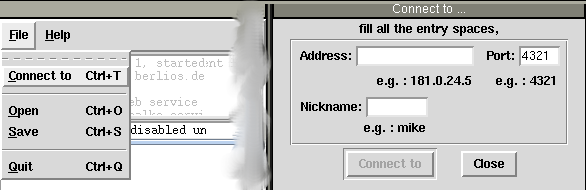
\includegraphics[angle=0,width=0.5\linewidth]{schemas/simples_menus_and_dialogs.png}
 \end{center}
 \label{fig:simplesmenusanddialogs}
 \caption{Simples menus and dialogs}
\end{figure}


\subsection{API}

\href{http://www.python.org/topics/tkinter/}{Tkinter}

\begin{description}
\item [Pros]
    \begin{itemize}
    \item Easy to include in the python distribution
    \item Ligthweigth (? compared to wxwindows ?)
    \item Python default gui, crossplatform
    \item Good coloring facilities
    \item Documented, easy API
    \item Full Unicode support
    \item Stable API
    \end{itemize}

\item [Cons]
    \begin{itemize}
    \item Manage text as a bidimensional object
    \item Ugly: The gui is not similar to the OS default one (this may \href{http://tcl.projectforum.com/tk/47}{change} in the future)
    \item Low mindshare among other programmers, wxPython seems to be the mainstream python gui programming toolkit nowadays
    \item Increasingly few projects using it and as such there is less people reporting bugs, etc. (development is not too active lately
    \item But anyway we believe we should keep on using tkinter for the first release and see how things play along. Provided we honour our intent of keeping GUI code clearly separated from concurrent/networking code, we should be safe
    \end{itemize}
\end{description}

\fbox{\begin{minipage}[c]{\linewidth}   
\emph{Note}:the gui code implementation should be as well defined and separated as possible to allow future implementations using diferent gui engines (natives, scintilla, etc.)
\end{minipage}}
%@nonl
%@-node:rodrigob.20040908010357.2:Gui
%@-others

\end{document}
%@nonl
%@-node:rodrigob.20040908003956.1:@thin doc/design_proposal.tex
%@-leo
